\documentclass[11pt, oneside, a4paper]{article}
\usepackage{ifpdf}
\usepackage{graphicx}
\usepackage[colorlinks,bookmarksopen,linkcolor=black,pdfauthor={Vikram},urlcolor=blue]{hyperref}
\usepackage[colorlinks,bookmarksopen]{hyperref}
\usepackage[hmargin=1.5cm,vmargin=2.5cm]{geometry}
\usepackage{algorithmic}
\usepackage{algorithm}
\begin{document}
\begin{center}
\textbf{VISVESWARAYA TECHNOLOGICAL UNIVERSITY}
\end{center}
\begin{center}
\textbf{BELGAUM}\\
\thispagestyle{empty}
\begin{figure}[htb]
\begin{center}
\ifpdf

\includegraphics[scale=0.50]{vtu.png}
\else
\fi
\end{center}
\end{figure}
\textbf{SRI JAYACHAMARAJENDRA COLLEGE OF ENGINEERING, }
\textbf{MYSORE-570006}\\
\textsc{department of computer science and engineering}
\end{center}
\begin{figure}[htb]
\begin{center}
\ifpdf

\includegraphics[scale=0.30]{./logo.png}
\else
\fi
\end{center}
\end{figure}
\begin{center}
\textbf{\underline{Report on}}\\
\textsc{\\IMPLEMENTATION OF B$^+$-TREE\\}
\emph{\\Guidance of}\\
\textbf{\\N.R. PRASHANTH}\\
\textit{Professor}\\
\textit{Department of CS$\&$E, SJCE, Mysore.}\\
\vspace{1in}
\textbf{\underline{Done By:}}\\
\textsc{\\VIKRAM T.V.}\\
5th Semester,\\ Computer Science and Engineering,\\
S.J.C.E, Mysore\\
\title {IMPLEMENTATION OF B$^+$-TREE\\}
\end{center}
\newpage
\thispagestyle{empty}
\tableofcontents
\newpage
\pagenumbering{arabic}

\twocolumn
\section{Introduction}
A B$^+$-tree (Bplus Tree) is a type of tree which represents sorted data in a way that allows for efficient insertion, retrieval and removal of records, each of which is identified by a key. It is a dynamic, multilevel index, with maximum and minimum bounds on the number of keys in each index segment (usually called a "block" or "node").  The primary value of a B$^+$-tree is in storing data for efficient retrieval in a block-oriented storage context — in particular, filesystems as B$^+$-trees have very high fanout (typically on the order of 100 or more), which reduces the number of I/O operations required to find an element in the tree.

Each nonleaf node in the tree has between $\lceil$\emph{n}/2$\rceil$ and \emph{n} children, where \emph{n} is fixed for a particular tree.  Although there is a overheads in insertion, deletion operations and space, the performance benefits of B$^+$-tree allows it to be used in most of the applications.

\section{Structure of B$^+$-Tree}
A typical B$^+$-tree node contains \emph{n} pointers P$_1$, P$_2$, $\ldots$, P$_\emph{n}$ and \emph{n} - 1 search-key values K$_1$, K$_2$, $\ldots$, K$_\emph{n}$.  The search-key values within a node are in sorted order, that is if i $<$ j, then K$_i$ $<$ K$_j$.  The typical node of B$^+$-tree is as shown in figure 1.

\begin{figure}[htb]
\begin{center}
\ifpdf
	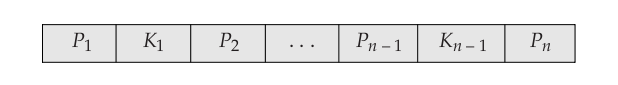
\includegraphics[scale=0.42]{./typicalBplusNode.png}
\else
\fi
\caption{Typical B$^+$-Tree Node}
\label{fig:1}
\end{center}
\end{figure}

\subsection{Structure of a Leaf Node}
For i = 1, 2, . . . , n − 1, pointer P$_i$ points to either a file record with search-key value K$_i$ or to a bucket of pointers, each of which points to a file record with search-key value K$_i$.  The last pointer points to the next leaf node in the tree.  Figures 2 and 3 taken from \cite{Korth} illustrates the usage of leaf nodes and the typical tree.
\begin{figure}[htb]
\begin{center}
\ifpdf
	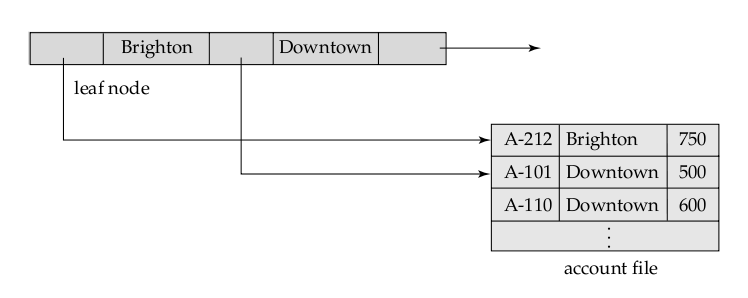
\includegraphics[scale=0.35]{./leafNode.png}
\else
\fi
\caption{Leaf Node with pointers pointing to records}
\label{fig:2}
\end{center}
\end{figure}
\begin{figure}[htb]
\begin{center}
\ifpdf
	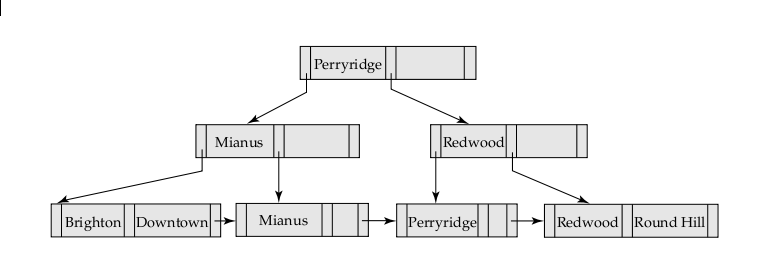
\includegraphics[scale=0.37]{./bplusTree.png}
\else
\fi
\caption{B$^+$-Tree}
\label{fig:3}
\end{center}
\end{figure}

During implementation, there should be a cast of the pointers while use in leaf nodes as those pointers point to records.  Figure 3 clearly shows the n$^th$ pointer pointing to the next leaf node and this allows for efficient sequential processing of the file.  Each leaf node can hold upto \emph{n} - 1 values and can contain as few as $\lceil$(\emph{n} - 1)/2$\rceil$ values.  Also, if L$_i$ and L$_j$ are leaf nodes and i $<$ j, then every search-key value in L$_i$ is less than every search-key value in L$_j$ . 

\subsection{Structure of non-Leaf nodes}
The structure of nonleaf nodes is the same as that for leaf nodes, except that all pointers are pointers to tree nodes.  A nonleaf node may hold up to \emph{n} pointers, and must hold at least $\lceil$\emph{n}/2$\rceil$ pointers.  Consider a nonleaf node containing \emph{m} pointers.  For i = 2, 3, . . . , m − 1, pointer P$_i$ points to the subtree that contains search-key values less than K$_i$ and greater than or equal to K$_i − 1$ . Pointer P$_m$ points to the part of the subtree that contains those key values greater than or equal to K$_m − 1$, and pointer P$_1$ points to the part of the subtree that contains those search-key values less than K$_1$.

Also, unlike other nonleaf nodes, the root node can hold fewer than $\lceil$\emph{n}/2$\rceil$ pointers, but it should hold at least two pointers, unless the tree consists of only one node.  Figure 3 shows a complete B$^+$-Tree with leaf and nonleaf nodes and \emph{n} = 3.  It is a B$^+$-Tree (Balanced plus tree) for an account file arranged alphabetically with path length 2.

\section{Querying B$^+$-Tree}
In order to search find all records with a search-key value of V, we first examine the root node, looking for the smallest search-key value greate than V and suppose this value is K$_i$, we follow the pointer P$_i$ to reach another node.  If there is no such value, then k $\ge$ K$_\emph{m} - 1$, where \emph{m} is the number of pointers in the node and hence follow P$_m$ to another node.  In the reached node, we again search for a smallest search-key value greater than V, and follow the corresponding pointer and eventually reach a leaf-node.  In the leaf-node, if search-key value K$_i$ equals V, then pointer P$_i$ directs to desired record or bucket of pointers.  If value of V is not found in leaf node, no record with key value V exists.

The algorithm to query a B$^+$-Tree is given in algorithm 1.\\
\textbf{Time Complexity}:  If there are K search-key values in the file, the path is no longer than $\lceil$ log $_\emph{n}$$_/$$_2$(K)
$\rceil$.

\begin{algorithm}
\caption{Querying a B$^+$-Tree}
\label{alg1}
\begin{algorithmic}[1]
\STATE \textbf{procedure} find (\emph{value} V)
\STATE set C = root node
\WHILE {C is not a leaf node}
\STATE Let K$_\emph{i}$ = smallest search-key value, if any, greater than V
\IF {there is no such value}
\STATE Let \emph{m} = the number of pointers in the node
\STATE set C = node pointed to by P$_\emph{m}$
\ELSE
\STATE set C = the node pointed to by P$_\emph{i}$
\ENDIF
\ENDWHILE
\IF {there is a key value K$_\emph{i}$ in C such that K$_\emph{i}$ = V}
\STATE pointer P$_\emph{i}$ directs us to the desired record or bucket
\ELSE
\STATE no record with key value \emph{k} exists
\ENDIF
\end{algorithmic}
\end{algorithm}

\section{Insertion to a B$^+$-Tree}
Insertion is a bit more complicated than finding a search-key.  We need to split a node that becomes too large as the result of an insertion.  Furthermore, when a node is split, we must ensure that balance is preserved.  Using the same technique as for lookup, we find the leaf node in which the search-key value would appear. If the search-key value already appears in the leaf node, we add the new record to the file and, if necessary, add to the bucket a pointer to the record. If the search-key value does not appear, we insert the value in the leaf node, and position it such that the search keys are still in order. We then insert the new record in the file and, if necessary, create a new bucket with the appropriate pointer.\\
\textbf{Splitting a node}:  We take the \emph{n} search-key values (the \emph{n} - 1 values in the node plus the value being inserted), and put the first \emph{n}/2 in the existing node and the remaining values in a new node. The new node must also be inserted to the tree such that the new node has the same parent as that of the existing node otherwise the parent node also needs to be split to make room for the new node.  The split of root makes the tree deeper by one level.

Consider the insertion of a key-value, pointer pair (V, P) to the B$^+$ index.  The general idea is to identify the leaf-node \emph{l} that holds the pair, and if a split results, insert the new node into the parent of node \emph{l}.  If this insertion too results in a split, proceed recursively up the tree, until no new split occurs or new root is created.  Algorithms 2 and 3 give the pseudocodes for \emph{insert}, \emph{insert$\_$in$\_$leaf} and \emph{insert$\_$in$\_$parent} respectively.  In the pseudocode, L, N, P and T denote pointers to nodes, with L being used to denote a leaf-node.  L.K$_i$ and L.P$_i$ denote the i$^t$$^h$ value and the i$^t$$^h$ pointer in node L, respectively. 'T' is a temporary that holds the contents of the node to be split.  In the case of leaf nodes, the pointer to an entry actually precedes the key value, so the leaf node actually stores P before V . For internal nodes, P is stored just after V.

\begin{algorithm}
\caption{Insertion into B$^+$-Tree - main routine}
\label {alg2}
\begin{algorithmic}[1]
\STATE \textbf{procedure} insert (\emph{value} K, \emph{pointer} P)
\STATE find the leaf node L that should contain key value K
\IF {L has less than \emph{n} - 1 key values}
\STATE insert$\_$in$\_$leaf (L, K, P)
\ELSE
\STATE /* L has \emph{n} - 1 key values already, split it */
\STATE Create node L'
\STATE Copy L.P$_1$, \ldots, L.K$_\emph{n}$$_-$$_1$ to a block of memory T that can hold \emph{n} (pointer, key-value) pairs
\STATE insert$\_$in$\_$leaf (T, K, P)
\STATE Set L'.P$_\emph{n}$ = L.P$_\emph{n}$; Set L'.P$_\emph{n}$ = L'
\STATE Erase L.P$_1$ through L.K$_\emph{n}$$_-$$_1$ from L
\STATE c = $\lceil$\emph{n}/2$\rceil$  /* c holds the ceil value of \emph{n}/2 */
\STATE Copy T.P$_1$ through T.K$_\emph{c}$ from T into L starting at L.P$_1$
\STATE Copy T.P$_c$$_+$$_1$ through T.K$_\emph{n}$ from T into L' starting at L'.P$_1$
\STATE Let K' be the smallest key-value in L'
\STATE insert$\_$in$\_$parent (L, K', L')
\ENDIF
\end{algorithmic}
\end{algorithm}

\begin{algorithm}
\caption{Pseudocodes for insertion in leaf and parent}
\label{alg3}
\begin{algorithmic}[1]
\STATE \textbf{procedure} insert$\_$in$\_$leaf (\emph{node} L, \emph{value} K, \emph{pointer} P)
\IF {K is less than L.K$_1$}
\STATE insert P, K into L just before L.P$_1$
\ELSE
\STATE Let K$_\emph{i}$ be the least value in L that is less than K
\STATE insert P, K into L just after T.K$_i$
\ENDIF
\STATE
\STATE \textbf{procedure} insert$\_$in$\_$parent (\emph{node} N, \emph{value} K', \emph{pointer} N')
\IF {N is the root of the tree}
\STATE create new node R containing N, K', N' /* N and N' are pointers */
\STATE make R the root of the tree
\STATE \textbf{return}
\ENDIF
\STATE Let P = parent (N)
\IF {P has less than \emph{n} pointers}
\STATE insert (K', N') in P just after N
\ELSE
\STATE /* Split P */
\STATE Copy P to a block of memory T that can hold P and (K', N')
\STATE Insert (K', N') into T just after N
\STATE Erase all entries from P; Create node P'
\STATE c = $\lceil$\emph{n}/2$\rceil$  /* c holds the ceil value of \emph{n}/2 */
\STATE Copy T.P$_1$ \ldots T.P$_\emph{c}$ into P
\STATE Let K'' = T.K$_\emph{c}$
\STATE Copy T.P$_\emph{c}$$_+$$_1$ \ldots T.P$_\emph{n}$$_+$$_1$ into P'
\STATE insert$\_$in$\_$parent (P, K'', P')
\ENDIF
\end{algorithmic}
\end{algorithm}

The above alogrithms were directly implemented with the necessary routines.

\section{Sample Run}
A sample run of the B$^+$ tree with size 5 and 10 elements resulted in the tree as shown in figure 4.  The sentinel value 999999 is used to generate random numbers for insertion.  Another run with size 5 and 10 elements is shown in figure 5.  Clearly, as the size decreases, the height of the tree increases and thus the search time becoming more.

\begin{figure}[htb]
\begin{center}
\ifpdf
	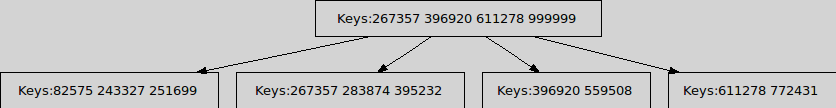
\includegraphics[scale=0.40]{./bplusSize5.png}
\else
\fi
\caption{B$^+$ Tree with size 5}
\label{fig:4}
\end{center}
\end{figure}

\begin{figure}[htb]
\begin{center}
\ifpdf
	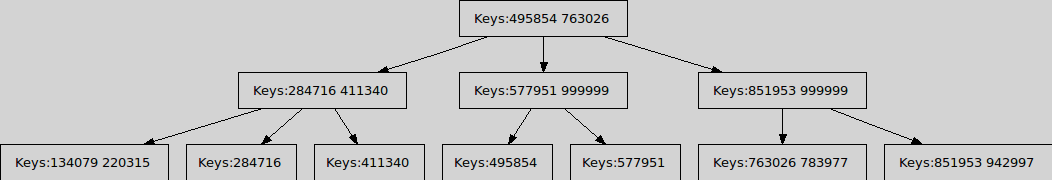
\includegraphics[scale=0.45]{./bplusSize3.png}
\else
\fi
\caption{B$^+$ Tree with size 3}
\label{fig:5}
\end{center}
\end{figure}

\begin{thebibliography}{10}
\bibitem[Silberschatz-Korth]{Korth} Abraham Silberschatz, Korth H.F., Sudarshan S., \emph{Database System Concepts}, Fifth Edition, McGRAW-HILL, 2006.
\end{thebibliography}

\end{document}